% Name: Surfaces by genus
% Description: The sphere, the torus, and the double torus, closed surfaces of genus 0, 1, and 2, with their Euler characteristics 2, 0, and −2.
% Tags: genus, Euler characteristic, closed surfaces, torus, topology

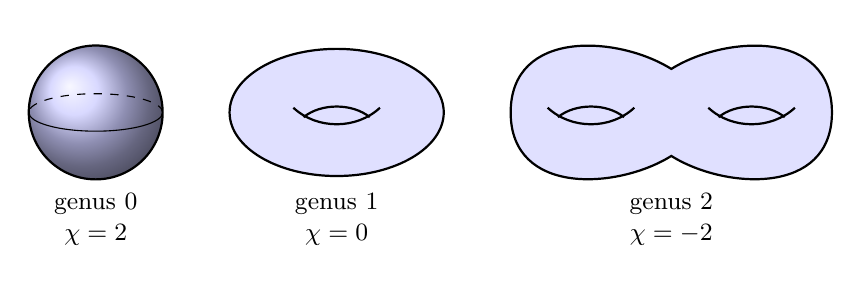
\begin{tikzpicture}[scale=0.85, thick, every node/.style={font=\small},
    % A hole: the lower curve shows its near rim, the shorter upper curve its far rim
    pics/hole/.style={code={
      \draw (-0.55,0.06) .. controls (-0.25,-0.22) and (0.25,-0.22) .. (0.55,0.06);
      \draw (-0.42,-0.06) .. controls (-0.2,0.12) and (0.2,0.12) .. (0.42,-0.06);}}]
  \shade[ball color=blue!20] (0,0) circle (1);
  \draw (0,0) circle (1);
  \draw[thin] (-1,0) arc (180:360:1 and 0.28);
  \draw[thin, dashed] (1,0) arc (0:180:1 and 0.28);
  \draw[fill=blue!12] (3.6,0) ellipse (1.6 and 0.95);
  \pic at (3.6,0) {hole};
  \draw[fill=blue!12] (6.2,0) .. controls (6.2,1.25) and (7.8,1.15) .. (8.6,0.65) .. controls (9.4,1.15) and (11,1.25) .. (11,0) .. controls (11,-1.25) and (9.4,-1.15) .. (8.6,-0.65) .. controls (7.8,-1.15) and (6.2,-1.25) .. cycle;
  \pic at (7.4,0) {hole};
  \pic at (9.8,0) {hole};
  \foreach \x/\g/\c in {0/0/2, 3.6/1/0, 8.6/2/-2} \node[align=center] at (\x,-1.6) {genus \g\\$\chi = \c$};
\end{tikzpicture}
